\documentclass[a4paper,12pt]{article}
%Packet section
\usepackage[utf8]{inputenc}
\usepackage[style=ieee]{biblatex}
\usepackage{csquotes}
\usepackage[top=2.5cm,bottom=2.5cm,left=2cm,right=2cm]{geometry}
\usepackage[english]{babel}
\usepackage{float}
\usepackage{caption}
\usepackage{pdfpages} % Para insertar la portada en formato PDF.
\usepackage[hidelinks]{hyperref} % Para urls.
\usepackage{longtable} % Para tablas largas.
\usepackage{graphicx} % Para cargar imagenes
\usepackage{titlesec}
\usepackage{fancyhdr}
\usepackage[parfill]{parskip}
\usepackage[acronym,nogroupskip]{glossaries}
\usepackage{todonotes}
\usepackage{dirtree}
\usepackage{subcaption}
\usepackage{mathtools}
\usepackage{amsmath}
\usepackage{multirow}
\usepackage{algpseudocodex}
\usepackage{algorithm}
\usepackage{listings}
\usepackage{bytefield}
\raggedbottom

\addbibresource{ArchServicePlatforms.bib}

%Eliminar la sangría y otros ajustes de los headers
\setlength{\parindent}{0px}
\setlength{\headheight}{13.07225pt}
%Glosaries
\makenoidxglossaries

\newacronym{iot}{IoT}{Internet of Things}
\newacronym{mec}{MEC}{Mobile Edge Computing}
\newacronym{lorawan}{LoRaWAN}{Long Range Wide Area Network}
\newacronym{ism}{ISM}{Industrial, Scientific and Medical}
\newacronym{ir}{IR}{InfraRed}
\newacronym{uv}{UV}{UltraViolet}
\newacronym{pir}{PIR}{Passive InfraRed}
\newacronym{rfid}{RFID}{Radio Frequency Identification}
\newacronym{5g}{5G}{Fifth Generation of mobile communications}
\newacronym{saas}{SaaS}{Software as a Service}
\newacronym{mcu}{MCU}{MicroController Unit}
\newacronym{lln}{LLN}{Low power lossy Networks}
\newacronym{ppm}{PPM}{Parts Per Million}
\newacronym{ble}{BLE}{Bluetooth Low Energy}
\newacronym{rpc}{RPC}{Remote Procedure Call}
\newacronym{mvvm}{MVVM}{Model-View-ViewModel}

\renewcommand*\glspostdescription{\hfill}
\newcommand\acrfullr[2][]{\acrshort[#1]{#2} (\acrlong[#1]{#2})}


%New page styles
\fancypagestyle{specialpage}{
  \fancyhf{}
  \fancyhead[L]{}
  \fancyhead[R]{\textit{GLOSARY}}
  \fancyfoot[L]{}
  \fancyfoot[OR]{\thepage}
}
\fancypagestyle{indicefig}{
  \fancyhf{}
  \fancyhead[L]{}
  \fancyhead[R]{\textit{LIST OF FIGURES AND TABLES}}
  \fancyfoot[L]{}
  \fancyfoot[R]{\thepage}
}
\fancypagestyle{abstract}{
    \fancyhf{}
    \renewcommand{\headrulewidth}{0pt} % Asegurarse de que la barra negra también se elimine en esta página
    \fancyfoot[EL]{\thepage}
    \fancyfoot[OR]{\thepage}
}

%Tools to write code directly into the document.
\lstset{
    language=C++,         
    basicstyle=\ttfamily,
    numbers=left,
    numberstyle=\tiny,
    stepnumber=1,
    frame=single,
    tabsize=4,
    breaklines=true,
    captionpos=b,
    showspaces=false,
    showstringspaces=false
}


\title{Architectures and Service Platforms: Final Project}
\author{Group 3}
\date{February 2025}

\begin{document}
\begin{titlepage}
    \raggedleft
    \rule{2pt}{\textheight}
    \hspace{0.05\textwidth}
    \parbox[b]{0.9\textwidth}{
            {\Huge\bfseries FarmRisk}\\[\baselineskip] % Title
            {\Large\textit{An intelligent manager for perimetral farming}}\\[6\baselineskip] % Subtitle or further description
        
        \begin{center}
            
\includegraphics[width=0.6\textwidth]{images/logo2.png} % Replace with the path to your image
        \end{center}
        
        \vspace{0.1\textheight}
        {\Large\textsc{Diego\ Aceituno\vspace{0.01\textheight}\\
                        Renato\ Luigi Barra\vspace{0.01\textheight}\\
                        Dennis\ Tanda}}\\[1.5\baselineskip]
        \vspace{0.01\textheight}
        
        {\noindent\large Architectures and Service Platforms: Final Project}\\
        {\noindent\large Fall 2024}\\
    }
\end{titlepage}
\clearpage
\pagenumbering{roman}
\pagestyle{fancy}
\fancyfoot{}
\fancyhead[L]{}
\fancyfoot[L]{}
\fancyfoot[R]{\thepage}
\setcounter{tocdepth}{2}
\fancyhead[R]{\textit{Contents}}
\tableofcontents
\clearpage
\thispagestyle{indicefig}
\listoffigures
\listoftables
\clearpage
\section*{Glosary} % Glosario
\thispagestyle{specialpage}
\printnoidxglossary[style=list,type=\acronymtype,title=] % Acrónimos
\clearpage
\pagenumbering{arabic}
\fancyhead[R]{\textit{Introduction}}
\section{Introduction}

In recent years, \textit{Smart Farming} projects have been growing in popularity as a method to solve the challenges that the agriculture sector is facing in the last decades. 
This projects are based around the \acrfullr{iot} domain, in which sensors and actuators are connected and coordinated to obtain data to represent the real world, this data can 
later be processed to make decisions that will make the farmers life easier.

One of the problems that \textit{Smart Farming} deals with is the real-time protection of crops from different risks. This risks can go from natural 
risks such as wild fires, to wild animals trespassing fences to feed on the crops. IoT systems can also be applied to this problems, detecting in real-time 
these situations and obtaining all the information related to these events. 

Considering that the topic requires fast-response times, new technologies such as \acrfullr{mec} in combination with \textit{Cloud Computing} can be applied to 
process the data as closest as possible to the main use case. This Edge solutions can aggregate all the data from the sensors and, with the help of 
algorithms for decision making, calculate the best possible response in the fastest way possible.


Using this technologies, this document presents the design of a system for the risks management in crops of Madrid, Spain. 

These rural areas in the lasts decades have been declining in population. This creates two problems in relation to fire risks:
\begin{enumerate}
    \item The depopulation of land creates areas with higher risk of fires\cite{Yanosolo}, where intentional fires can be created and extend faster due to the heavy amount of fuel.
    \item Farmers now need to be aware of these areas in case a fire appears.
\end{enumerate}

In addition to the above mentioned, the risk of animal intrusion increases\cite{importanciacazaEspana}, as the perimetral limits of this crops is now uncontrolled.

To achieve the objective mentioned above, \acrshort{iot} technologies are be integrated with edge computing to create a fast-response system.
\todo[inline]{Poner información resumida sobre los casos de uso que afronta este sistema}
\clearpage
\fancyhead[R]{\textit{System Description}}
\section{System Description}

The FarmRisk system can be divided considering the main two risks presented before:

\begin{itemize}
    \item The risk of fire hazards in the vicinities of the farm need to be detected, in order to ensure save operations. To do this, fire and smoke sensors are used to detect early signs of fire. This data will be 
    sent to the middleware and a decision system will infer the presence of fire. If any fire is detected, the farmer will be notified\todo{ponemos aquí lo de telegram?}, indicating the proximity and the location of 
    the detection.
    \item Secondly, if any signs of wild animal presence are detected near the limits of the farm, information will be sent to the edge platform. This information will be used to decide the possible actuator execution. 
    If it is decided that an animal has been detected, it will be notified to the user. To detect this presence, sensors of presence and accelerometers are used, this allows for the coverage of bigger distances without the 
    need of extra budget.
\end{itemize}

To integrate all the sensing of the farm's border, an specific node connects all the sensors and is in charge of sending information to the communications gateway. This sensor will be placed every $50m$ in the border.

This information will be forwarded to the edge computing platform., implemented using Thingsboard. When the data arrives, it is processed (while being logged) in order to determine possible actions or alarms that need to be 
executed.

The edge computing platform will also communicate with a system that allows for weather condition information, using the \texttt{AEMET API}\cite{AEMETOpenDataAgencia}. This information will be used to determine possible 
fire risks in near future, notifying the farmer that soil moisture need to be improved.

Finally, the system will allow the possibility of two type of users: admin or worker. The worker will only be able to receive alerts and see the current status of the system, while the admin user will be able to command the 
network, stopping the alert system, responding to alerts, etc.



\clearpage
\fancyhead[R]{\textit{Project Scope}}
\section{Project Scope}
This project addresses multiple use cases on a farm, which will be detailed in the following chapters through UML diagrams and a 
Project Requirement Analysis. However, due to time and resource constraints, it is not feasible to implement the entire project 
with all its functionalities. Consequently, the project will incorporate both real and simulated hardware.

A real embedded system will be developed, equipped with PIR sensors for presence detection, accelerometers to monitor movements on
the crop field fences, soil moisture sensors to assess dryness levels, and a GPS module to provide information about the device’s current location.

Additionally, real meteorological data will be obtained through requests to the WeatherCast API [], enabling the analysis of wildfire probabilities in the monitored area.

To complement this, the system will simulate hardware responsible for fire detection. By using software simulations of fire detection
sensors, combined with data on climatic conditions and physical soil factors, it will be possible to validate alerts generated in response
to potential wildfire risks or active fire detections.

Due to the project’s limitations and scope, the proof of concept will be conducted on a small scale, focusing on achieving the course objectives.
These objectives will be addressed by utilizing both real and simulated hardware, where periodic events will be sent regarding soil and weather conditions,
as well as sporadic events in the event of potential animal detection via the PIR sensor or accelerometers on the fences.  Moreover, the project will
include alarm systems to detect animal presence, imminent wildfire risks, or the occurrence of an active fire. This approach ensures the main goals of the course are met.

\todo[inline]{TODO: Agregar referencia API tiempo}

\todo[inline]{TODO: Poner Figura descriptiva generica}
\clearpage
\fancyhead[R]{\textit{Previous Works}}
\section{Previous Works}

Some of the topics covered in this project follow some existing research lines line:
\begin{itemize}
    \item Wireless sensor networks.
    \item Fire detection sensors.
    \item Animal intrusion detection.
\end{itemize}

In relation to this, there are already some examples of working projects that focus on 
protecting the crops from the external risks mentioned in earlier chapters. These projects achieve solutions 
using current technologies, which will be analyzed in this chapter to understand the \textit{state of the art}. 

The analysis of this projects results in a classification into three main types of solution design: \acrshort{iot}-based systems, 
solutions that incorporate AI, and finally hybrid systems.

\subsection{Type of systems}
\subsubsection*{\acrshort{iot}-based solutions}

The Internet of Things has become an important tool for detecting risks. Sensors and embedded systems are used 
to collect real-time information and analyze the presence of wild animals or fires in the proximity of controlled areas.

These solutions architecture contain the next elements:
\begin{itemize}
    \item A set of intercommunicated nodes that obtain information through and send data through a wireless network.
    \item A middleware layer to operate and integrate all this information for the user-level applications.
    \item End-User application layer.
\end{itemize}

\subsubsection*{AI-based solutions}

Solutions using AI and machine learning are effective for animal classification and recognition, and this usage has been extended to detect 
behavior, like farm intrusions\cite{PDFWildAnimals}. These systems are typically designed to process images collected by cameras and maybe 
additional information from sensors, identifying patterns that allow different species or even animals and humans to be distinguished.

For instance, algorithms such as YOLOv8 have proven highly effective at detecting animals in real-time using image 
analysis\cite{WildAnimalDetection}. These systems divide images into grids, simultaneously predict bounding boxes, and assign probability to detected 
classes. These tools can also be used to process thermal images and detect fires. 

The main drawback of these systems is the training stage with large pre-labeled data sets, needing a preparation of training data 
in order to achieve the results expected. This step is also very heavy in power consumption, and, depending on the objective, it may not be needed.

\subsubsection*{Hybrid solutions}

This is the main paradigm being followed by the \acrshort{iot} industry in order to solve problems. These architectures 
integrate AI capabilities into the middleware to offer more complete and adaptable solutions.

An example of this kind of system is a project that combines PIR sensors and thermal cameras to collect data. This data is processed 
in the middleware by machine learning models to classify the type of animal detected, reducing the number of false positives and optimizing 
response, as specific measures can be applied depending on the identified species\cite{StudyMethodsAnimal}.

\subsection{Wireless Sensor Networks}

To monitor the presence of animals or fires, different devices that include sensors can be interconnected with each other to obtain 
information of the real world.

To transmit this data, different wireless technologies are used, and there can be more that one technology for any 
implementation, as it is device-dependent. 

The technology selected depend on different parameters:
\begin{itemize}
    \item Speed needed.
    \item Need for a license-free environment, using the \acrfullr{ism} band.
    \item Maximum number of nodes interconnected.
    \item Size of data sent and period of that data.
    \item Is low power consumption needed on the node?.
\end{itemize}
Some of the mainly used technologies are Wi-Fi, mobile networks (LTE-M or NB-IoT), \acrfullr{lorawan} or SigFox. Some of the key characteristics of this technologies can be seen in the next table.
\begin{table}[H]
    \begin{center}
        \begin{tabular}{p{0.10\textwidth} |  p{0.20\textwidth}  p{0.20\textwidth} p{0.20\textwidth} p{0.20\textwidth}}
            \hline
            \textbf{Param} & \multicolumn{1}{c}{\textbf{LoRaWAN}} & \multicolumn{1}{c}{\textbf{SigFox}} & \multicolumn{1}{c}{\textbf{NB-IOT}} & \multicolumn{1}{c}{\textbf{Wi-Fi}}\\
            \hline
            Range & \makecell{$\leq5$km (Urban)\\$\leq15$km (Rural)} & \makecell{$\leq10$km (Urban)\\$\leq50$km (Rural)} & \multicolumn{1}{c}{$\leq15$ km} & \multicolumn{1}{c}{$\leq40$ m}\\
            \hline
            Licensed band? & \multicolumn{1}{c}{No} & \multicolumn{1}{c}{No} & \multicolumn{1}{c}{Yes} & \multicolumn{1}{c}{No}\\
            \hline
            Data Rate & \makecell{37.5 kbps (LoRa) \\ 50 kbps (FSK)} & \makecell{100 bps (UL) \\ 600 bps (DL)} & \multicolumn{1}{c}{$\leq150$ kbps} & \multicolumn{1}{c}{Several MBps}\\
            \hline
        \end{tabular} 
    \end{center}
    \caption{Parameter differences between wireless network technologies}
    \label{ReqGeneral}
\end{table}

\subsection{Study on the sensors being used}
\todo[inline]{Poner un resumen de los tipos de sensores}.

\subsection{Middleware technologies}
\todo[inline]{Poner alguna parrafada, con un texto sobre thingsboard, nodered y kafka}.
\clearpage
\fancyhead[R]{\textit{Requirement Analysis}}
\section{Requirement Analysis}

\subsection{Stakeholder Analysis}

This project can affect several type of future users. This needs to be considered to stablish the scenarios the system will face. 

\begin{itemize}
    \item \textbf{Farmers}: The end users who will utilize the system to protect their crops and properties. The jobs these farmers carry out can differ, for example, one farmer can be the owner of the system 
    and others can just be workers that also need to access the system.
    \item \textbf{Maintenance Personnel}: If any problem appears, these users are responsible for maintaining the system and ensuring it's proper functioning.
    \item \textbf{Equipment and Sensor Suppliers}: Companies that supply necessary components, such as \acrfullr{mcu}, smoke, flame or motion sensors.
    \item \textbf{Internet Service Providers}: These companies supply the resources for edge computing and internet connectivity.
    \item \textbf{Governmental and Regulatory Organizations}: Entities that ensure the system complies with agricultural and safety regulations.
    \item \textbf{Agricultural Consultants}: Professionals who advise farmers on integrating and using the system in their agricultural practices.
    \item \textbf{Energy Suppliers}: Companies that provide energy solutions, such as solar panels, to power the system.
    \item \textbf{Local Community}: Neighbors and other local stakeholders who could indirectly benefit from the system's implementation.
    \item \textbf{Investors and Financiers}: Entities or individuals who provide the necessary funds for the system's development and implementation.
\end{itemize}

\subsection{Functional Requirements}

\subsection{Non-Functional Requirements}

\subsection{Operation Domain Requirements}

\begin{itemize}
    \item Interaction with the farm workers while maintaining compatibility with agricultural practices.
    \item Helping in the promotion of sustainable practices and efficient energy use.
    \item Compliance with agricultural and privacy regulations.
    \item Optimization of the use of agricultural resources.
\end{itemize}

\clearpage
\subsection{Quality attributes analysis and Impact analysis}

\begin{itemize}
    \item \textbf{Performance}:
        \begin{itemize}
            \item \textbf{Response time}: The system must process and respond to alerts in less than $1$ second.
            \item \textbf{Processing capacity}: It must handle multiple simultaneous events without degrading performance.
        \end{itemize}
    \item \textbf{Reliability}:
        \begin{itemize}
            \item \textbf{Availability}: The system must be operational at least $99 \%$ of the time.
            \item \textbf{Redundancy}: It must have backup mechanisms to ensure service continuity in case of failures.
        \end{itemize}
    \item \textbf{Security}:
        \begin{itemize}
            \item \textbf{Data protection}: All transmitted data must be encrypted.
            \item \textbf{Controlled access}: Only authorized users should be able to access and control the system.
        \end{itemize}
    \item \textbf{Scalability}:
        \begin{itemize}
            \item \textbf{Sensor expansion}: It must allow the addition of new sensors and actuators without significant changes.
            \item \textbf{User increase}: The system should support a growing number of users and connected devices. 
        \end{itemize}
    \item \textbf{Maintainability}:
        \begin{itemize}
            \item \textbf{Ease of updating}: The system must allow software updates without interrupting its operation.
            \item \textbf{Documentation}: There must be clear and detailed documentation to facilitate maintenance.
        \end{itemize}
    \item \textbf{Usability}:
        \begin{itemize}
            \item \textbf{User-friendly interface}: The interface must be intuitive and easy to use for people without technical knowledge.
            \item \textbf{Accessibility}: It must be accessible from different devices (mobile and computers).
        \end{itemize}
\end{itemize}

Based on the quality attributes presented above, each attribute has been classified according to its relevance and complexity within the system, as presented in \autoref{qualityPriorities}.

\begin{table}[H]
    \begin{center}
        \begin{tabular}{p{0.20\textwidth} |  p{0.35\textwidth}  p{0.35\textwidth} }
            \hline
            \textbf{Quality Attribute} & \multicolumn{1}{c}{\textbf{Relevance}} & \multicolumn{1}{c}{\textbf{Complexity}}\\
            \hline
            Response Time & \makecell{High} & \makecell{High}\\
            \hline
            High Processing & \makecell{High} & \makecell{Medium}\\
            \hline
            Availability & \makecell{High} & \makecell{High}\\
            \hline
            Redundancy & \makecell{High} & \makecell{Medium}\\
            \hline
            Data Protection & \makecell{Low} & \makecell{Low}\\
            \hline
            Controlled Access & \makecell{High} & \makecell{Low}\\
            \hline
            Sensor Expansion & \makecell{High} & \makecell{Medium}\\
            \hline
            User Increase & \makecell{Medium} & \makecell{High}\\
            \hline
            Ease of Updating & \makecell{High} & \makecell{High}\\
            \hline
            Documentation & \makecell{Medium} & \makecell{Medium}\\
            \hline
            Friendly UI & \makecell{High} & \makecell{Medium}\\
            \hline
            Accessibility & \makecell{High} & \makecell{Medium}\\
            \hline
        \end{tabular} 
    \end{center}
    \caption{Prioritization of Quality Attributes Based on Relevance and Complexity}
    \label{qualityPriorities}
\end{table}
\clearpage
\fancyhead[R]{\textit{System Architecture}}
\section{System Architecture}

This system mainly focus in the interconnection and interoperability of different elements. 
To achieve this, an architecture was designed in response to the requirements.

A general overview of the proposed architecture can be seen in \autoref{fig:architecture}.

\begin{figure}[H]
    \centering
    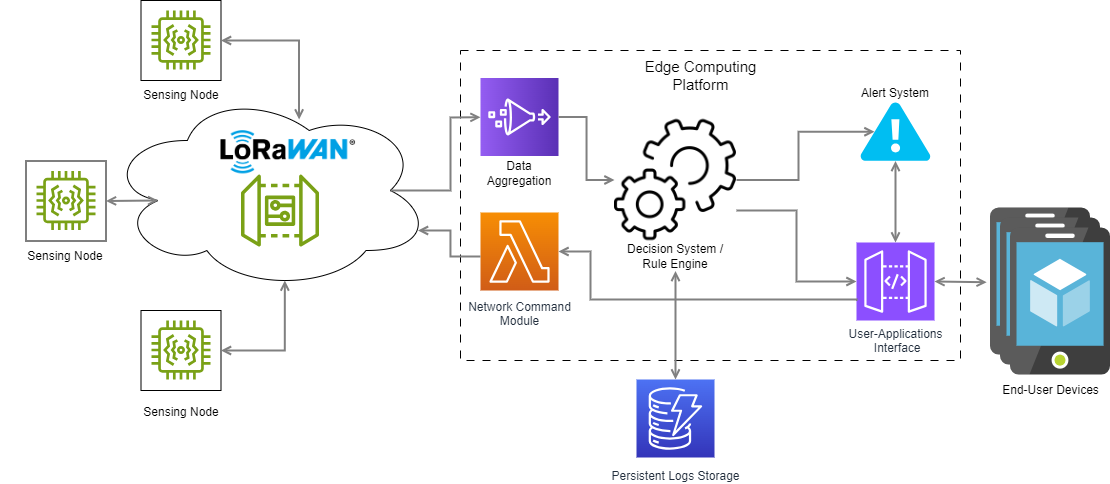
\includegraphics[width=1\textwidth]{./images/6/generalArchitecture.png}
    \caption{General architecture design for the proposed system.}
    \label{fig:architecture}
\end{figure}

Thanks to the research done, the selection for the intercommunication of the nodes with the edge platform 
will be done using \acrshort{lorawan}. This protocol ensures good coverage in rural areas, moreover, it ensures 
scalability in the system designed. The connection is done with lora from the nodes to the gateway. 
This gateway connects to the edge computing platform with IP technologies to send all the data from the nodes. 
Finally, this data will be collected in the data aggregation module, which will allow information coming from other 
wireless technologies or other \acrfullr{lln}.

When all the data is aggregated, it will pass through the rule engine module. This step analyzes the data in search 
for patterns that indicate the existence of a fire or will animal near the system. All these processing is logged into a 
persistent data storage that can serve as a knowledge base for future projects. 

If a fire or wild animal is detected, a set of actions are done, this is done through the alarm system of the edge platform and 
the User-Application interface. These modules allows for interaction with the users, allowing different functionalities like:
\begin{itemize}
    \item Access from mobile applications to the processed data.
    \item Real-Time alarm and registration of events.
    \item Allowing users to react, sending commands to the network to solve problems.
\end{itemize}


\clearpage
\fancyhead[R]{\textit{Implementation}}
\section{Implementation}
\clearpage
\fancyhead[R]{\textit{Testing and Validation}}
\section{Testing and Validation}
\subsection{Testing}
This part is the testing.

\clearpage
\subsection{Validation}

This part is validation.
\clearpage
\fancyhead[R]{\textit{Conclusions}}
\section{Conclusions and Future Work}
\subsection*{Conclusions}
The research done for this project shows the importance of \acrshort{iot} solutions in the farming industry. More specific, new solutions need 
to be achieved in the design of crop protection applications. And most importantly, fires are not the only risk that farm faces.

Some possible solutions that are being studied in this project are the use of \acrshort{pir} sensors in order to achieve a high level of 
power efficiency. If this reactive data is sent using low power wireless technologies like \acrshort{lorawan}, it can be use 
for new scenarios like machine learning, applied decision support algorithms and more. To support this, the use of \acrshort{mec} is mandatory.

In the first stage, the edge platform main functionalities and decision systems were implemented, along with simulated devices and dashboard solutions to 
give the user all the necessary information processed in a real-time manner.

In the second stage, the real hardware implementation of the nodes was achieved. In addition, an enhancement of the solution was made, building an application around the \acrshort{mec} platform in order to use the most common \acrshort{iot} 
devices, mobile phones. Finally, the possibility of commanding the network for cleaning tasks was added.

Finally all the necessary validations and test were made in order to check the required functionalities.

\subsection*{Future Work}

Due to the limitations in time, there are some good ideas that could apply to this project:
\begin{enumerate}
    \item The nodes need further enhancement in the selection of the \acrshort{mcu} in order to obtain the lowest possible power consumption. Also, an encapsulation design 
        for the nodes is needed.
    \item Due to the limitations, the targeted technology of \acrshort{lorawan} wasn't used and needs to be tested. A gateway would be needed before the Thingsboard platform.
    \item On of the key aspects that need to be tackled is the modification of the system in order to achieve full scalability. This 
        could be done creating a mission manager that controls the entities in ThingsBoard, allowing creation and expansion with new nodes in 
        an already existing farm.
    \item Finally, we propose a system that utilizes the knowledge extraction database combined with weather data\cite{AEMETOpenDataAgencia} in order to generate a predictor of 
        animal intrusion and fire hazards.
\end{enumerate}

\clearpage
\fancyhead[R]{\textit{References}}
\printbibliography[title={References}, heading=bibnumbered]

\end{document}